%% LaTeX2e class for student theses
%% sections/content.tex
%% 
%% Karlsruhe Institute of Technology
%% Institute for Program Structures and Data Organization
%% Chair for Software Design and Quality (SDQ)
%%
%% Dr.-Ing. Erik Burger
%% burger@kit.edu
%%
%% Version 1.3.3, 2018-04-17

\chapter{Applying \gls{RDF2Graph} to Wikidata}
\label{ch:RDF2Graph+Wikidata}

This chapter describes the changes that were made to \gls{RDF2Graph} and related software in the course of this thesis.
Some of them are general improvements unrelated to \gls{Wikidata} (\cref{sec:RDF2Graph+Wikidata:updates}),
some are motivated by the \gls{Wikidata} use case but still generally useful (\cref{sec:RDF2Graph+Wikidata:cyclic-graphs,sec:RDF2Graph+Wikidata:schema-reduction,sec:RDF2Graph+Wikidata:depth-limit}),
and some are specific to \gls{Wikidata} and result in a version of \gls{RDF2Graph}
that cannot be used for other RDF graphs (\cref{sec:RDF2Graph+Wikidata:Wikidata}).
All the changes are available in the source code repositories at
\url{https://github.com/lucaswerkmeister/RDF2Graph} and
\url{https://github.com/lucaswerkmeister/RDFSimpleCon},
in the \branchname{master} and \branchname{wikidata} branches;
some of them may also be merged into the upstream \gls{RDF2Graph} and \gls{RDFSimpleCon} repositories in the future.

\section{General \gls{RDF2Graph} Updates}
\label{sec:RDF2Graph+Wikidata:updates}

The \branchname{master} branch of the \gls{RDF2Graph} source code repository
has not seen any updates since 2015 (when \cite{vanDam2015} was published),
so some updates were needed to make the program run on newer software versions
and to target a more recent version of \gls{shex}.
Many of these were rather minor in nature,
but a few of the major ones concerning the \gls{shex} exporter are described in this section.
(I later noticed that the \gls{RDF2Graph} source code repository
also has a \branchname{dev} branch,
which has some more recent changes including a few fixes,
but most of them are not relevant to the issues discussed here.)

The final step of the \gls{shex} export was mostly rewritten from scratch.
This is the step that translates a \gls{json-ld} file describing the shapes of the schema
into a \gls{shexc} file;
the previous version did this using Jade,
a templating engine for \gls{html} documents (renamed to Pug in 2016),
constructing an \gls{html} document containing a single plain-text \lstinline[language=html]{<pre>} element,
then extracting this text from the document using an \gls{html}-to-text converter.
The new version directly produces the text from \gls{JavaScript}
and includes several improvements:
datatypes are now properly supported,
whereas the previous version only supported a handful of hard-coded \glspl{iri} as datatypes
and exported all other datatypes as if they were actually \glspl{shape};
prefixes are used everywhere in the output, highly improving readability;
and the output is sorted, making the whole generation process more deterministic
and thus making it easier to compare the results of multiple inference processes.

The syntax of the generated \gls{shexc} \glspl{schema}
also required some changes.
First, \gls{RDF2Graph} originally targeted \gls{shex} version 1.0
whereas the current release is version 2.0,
which introduced some syntactic changes
(e.~g. replacing some commas with semicolons).
Second, \gls{RDF2Graph} emitted syntax for an experimental, in-progress version of \gls{shex}
with support for inheritance between \glspl{shape}:
if, for example, the inferred \gls{schema} contained classes for both “human” and “person”,
and “human” was a subclass of “person” in the input data set,
then \gls{RDF2Graph} would declare that the “human” \gls{shape} extended the “person” \gls{shape}
and omit \glspl{predicate} from the “person” \gls{shape} in the “human” \gls{shape},
since those would be redundant with the \glspl{predicate} inherited from the “person” \gls{shape}.
This feature has not made it into any released version of \gls{shex} yet
(it can still be found in \branchname{on-shape-expression} branches of related repositories,
though the syntax has slightly changed:
it now uses the keyword \lstinline{EXTENDS} whereas \gls{RDF2Graph} used the symbol \lstinline{&}),
so the \gls{shex} exporter was changed to only mention the parent classes for a \gls{shape} in a comment,
and simplification step 4 (see \cref{sec:Background:RDF2Graph}) was disabled
so that the redundant \glspl{predicate} are included after all,
since they are no longer automatically inherited.

\section{Wikidata Support}
\label{sec:RDF2Graph+Wikidata:Wikidata}

This section outlines the general process that is used when running \gls{RDF2Graph} against data from \gls{Wikidata}
and then describes several changes to \gls{RDF2Graph} that were necessary to support this.
(The subsequent subsections correspond to those changes, not to the individual steps of the process.)

\subsection{Overall process, data download}
\label{subsec:RDF2Graph+Wikidata:Wikidata:download}

Usually, \gls{RDF2Graph} is run against a \gls{sparql} endpoint
which serves the \gls{rdf} graph for which one wants to infer the structure.
However, simply running \gls{RDF2Graph} against \acrfull{wdqs}, the public \gls{sparql} endpoint for \gls{Wikidata},
would mean attempting to infer a \gls{schema} from all of \gls{Wikidata},
which is neither the goal of this thesis
(that is to infer \glspl{schema} from a small set of exemplary \glspl{item})
nor even remotely feasible given the amount of data in \gls{Wikidata}
(for example, the 2018-08-20 full \gls{Wikidata} dump, uncompressed,
is \SI{309.7}{\giga\byte} large and \num{8316156305} lines long).

Instead, a process was set up which,
given a query which selects the exemplary \glspl{item},
downloads the related data for them and runs \gls{RDF2Graph} against it.
The process is outlined in \cref{fig:process}
and controlled by a Makefile in the \gls{RDF2Graph} repository,
so that after creating an \filename{\variable{example}.entities.sparql} file
with a \gls{sparql} query selecting the exemplary items,
it is sufficient to run \command{make \variable{example}.shex}
to run the entire process and generate the \gls{shex} file.

\begin{figure}
  \centering
  \begin{tikzpicture}
    \tikzstyle{file} = [rectangle, draw, rounded corners, text centered]
    \tikzstyle{pipe} = [style=file, dashed]
    \tikzstyle{directory} = [rectangle, draw, text centered]
    \tikzstyle{arrow} = [draw, -latex', right]

    \begin{scope}[node distance=2cm]
      \node[file] (entities) {\filename{\variable{example}.entities.sparql}};
      \node[file, below of=entities] (data) {\filename{\variable{example}.data.sparql}};
      \node[pipe, below of=data] (JSON) {\filename{\variable{example}.json}};
      \node[file, below of=JSON] (N-Triples) {\filename{\variable{example}.nt}};
      \node[directory, below of=N-Triples] (Fuseki) [align=center] {\dirname{\variable{example}-fuseki} \\ \texttt{http://localhost:3030/\variable{example}/query}};
      \node[directory, below of=Fuseki] (RDF2Graph) {\dirname{\variable{example}-results}};
      \node[file, below of=RDF2Graph] (ShEx) {\filename{\variable{example}.shex}};
      \node[file, below of=ShEx] (HTML) {\filename{\variable{example}.html}};
    \end{scope}

    \begin{scope}[every path/.style=arrow, midway]
      \path (entities) -- node {\command{sed}} (data);
      \path (data) -- node {\gls{wdqs}} (JSON);
      \path (JSON) -- node {\command{jq}} (N-Triples);
      \path (N-Triples) -- node {Fuseki} (Fuseki);
      \path (Fuseki) -- node {\gls{RDF2Graph}} (RDF2Graph);
      \path [dashed] (RDF2Graph.north east) to [out=30,in=330,looseness=5] node {\gls{RDF2Graph}, simplify} (RDF2Graph.south east);
      \path (RDF2Graph) -- node {\gls{shex} exporter} (ShEx);
      \path (ShEx) -- node {\command{pygmentize}} (HTML);
    \end{scope}
  \end{tikzpicture}
  \caption{An overview of the overall process.}
  \label{fig:process}
\end{figure}

First, the query selecting the exemplary \glspl{item} is transformed
into a query selecting all the required data,
using the Unix \command{sed} command.
The generated query selects all \glspl{statement} of the exemplary \glspl{item} (“direct \glspl{statement}”),
all \glspl{statement} of \glspl{item} which occur as values of the direct \glspl{statement} (“indirect \glspl{statement}”),
and all \PL{P31}{instance of} \glspl{statement} of \glspl{item} which occur as values of the indirect \glspl{statement}.
This query is run against \gls{wdqs},
which returns the results in \gls{json} format;
they are then piped into a script for the \command{jq} tool (“\gls{json} query”),
which transforms them into \gls{N-Triples} format,
and stored in an \gls{N-Triples} file.

Next, the Apache Jena Fuseki \gls{sparql} server is run locally,
serving the data from this \gls{N-Triples} file,
and as soon as it has finished loading the data file,
\gls{RDF2Graph} is run against this local \gls{sparql} endpoint for the main inference process,
including \gls{RDF2Graph}’s simplification step.
Once \gls{RDF2Graph} terminates, the Fuseki server is stopped.

Afterwards, the results from \gls{RDF2Graph} are available as a graph of classes with associated information,
and the \gls{RDF2Graph} \gls{shex} exporter is run to produce a \gls{shex} file.
If desired (\command{make \variable{example}.html}),
that file can also be turned into an \gls{html} file using the Pygments syntax highlighter,
which makes the \gls{shex} code more readable.

% TODO look over the subsections again.
% in general, each should first introduce a problem and then state my solution.
% some of them should also probably be longer than one paragraph

\subsection{Type predicates}
\label{subsec:RDF2Graph+Wikidata:Wikidata:predicates}

The most fundamental change to make \gls{RDF2Graph} support \gls{Wikidata}
was % TODO is?
to change the type predicates used.
\Gls{RDF2Graph} heavily relies on the type information of the RDF graph it inspects,
assuming a one-to-one mapping between classes and shapes,
and it uses the standard \glspl{predicate} \PName{rdf:type} and \PName{rdfs:subClassOf}
to determine the class of a subject and the superclasses of a class, respectively.
However, \gls{Wikidata} does not use these standard \glspl{predicate}:
the class(es) and superclass(es) of an item
are regular \glspl{statement} like any other \gls{Wikidata} \gls{statement},
using the \glspl{property} \PL{P31}{instance of} and \PL{P279}{subclass of}.
In the \gls{rdf} export, \PName{rdf:type} and \PName{rdfs:subClassOf} are only used
as part of the meta-model, % TODO meta-model? hm
assigning each item the class \PName{wikibase:Item}, a subclass of \PName{wikibase:Entity}.
To use the type information within the data instead of this meta-model,
\gls{RDF2Graph} was changed to use the \glspl{predicate} \PName{wdt:P31} and \PName{wdt:P279}
instead of \PName{rdf:type} and \PName{rdfs:subClassOf}.

\subsection{Data reduction}
\label{subsec:RDF2Graph+Wikidata:Wikidata:reduction}

During the data download step, some data is dropped from the \glspl{item}.
For one, the \glspl{label}, \glspl{description} and \glspl{alias} of an \gls{item} can make up a large portion of its data,
but are generally not interesting for \gls{shex} schemas,
since there is rarely more to say about them than
“an \gls{item} has one or more \glspl{label}, zero or more \glspl{description}, and zero or more \glspl{alias}”.
(A manually curated \gls{schema} might go beyond this –
perhaps requiring, for example, that \glspl{item} about Spanish municipalities have a label in Spanish –
but such details are beyond the ability of \gls{RDF2Graph} to infer.)
Additionally, \gls{Wikidata} \glspl{item} often have a number of \glspl{statement} listing external identifiers for the \gls{item}
(that is, identifiers in other databases for the same concept described by this \gls{item}):
for example, \gls{Wikidata}’s \Q{Q80} corresponds to \loc{no99010609} in the \gls{loc},
\viaf{85312226} in \gls{viaf},
\imdbName{nm3805083} in the \gls{imdb},
\TwitterAccount{timberners\_lee} on Twitter,
and dozens of other external identifiers.
All these external identifiers are technically just ordinary \glspl{statement},
but since they carry a rather different kind of information than other \glspl{statement},
they are sorted into a separate section when viewing the \gls{item} on the \gls{Wikidata} website.
To reduce the runtime of the \gls{RDF2Graph} inference process,
and to reduce clutter in the inferred \glspl{schema},
the \glspl{label}, \glspl{description}, \glspl{alias}, and external identifiers of an \gls{item}
are therefore excluded when downloading the data for a set of exemplary \glspl{item}.

\subsection{Full type hierarchy}
\label{subsec:RDF2Graph+Wikidata:Wikidata:hierarchy}

However, one unfortunate consequence of running \gls{RDF2Graph} against a reduced data set
is that \gls{RDF2Graph} cannot see the full type hierarchy of the classes involved:
for example, depending on how much data was downloaded,
it may or may not be aware that the classes \QL{Q112099}{island nation} and \QL{Q3624078}{sovereign state}
have a common superclass, \QL{Q7275}{state},
which reduces the available options during the simplification step. % TODO not happy with this phrasing
To mitigate this, \gls{RDF2Graph} was patched
to allow specifying an alternative \gls{sparql} endpoint for all queries that require a full view of the data,
and uses this alternative endpoint for the query to get all parent and child classes of a class.
The Makefile mentioned in \cref{subsec:RDF2Graph+Wikidata:Wikidata:download}
specifies the \gls{wdqs} \gls{sparql} endpoint for this option,
so that \gls{RDF2Graph} can learn the full class hierarchy around all relevant items % TODO is “learn” the right word?
even when running against a subset of \gls{Wikidata}. % TODO “subset of Wikidata”? not quite happy with that phrasing

\subsection{Simplification}
\label{subsec:RDF2Graph+Wikidata:Wikidata:simplification}

The simplification process also required some changes to support \gls{Wikidata}.
Originally, \gls{RDF2Graph} would merge all classes into their superclass,
almost completely unconditionally,
stopping only at the root class \PName{owl:Thing}.
This was much too aggressive for \gls{Wikidata}:
not only does \gls{Wikidata} have a different root class (\QL{Q35120}{entity}),
but it also has a complex hierarchy of abstract classes below that root class,
and merging other classes into those abstract classes
(like \QL{Q151885}{concept}, \QL{Q7184903}{abstract object} or \QL{Q830077}{subject})
would not result in useful schemas.
Therefore, step 2 in the simplification process was adapted
to add a number of \gls{Wikidata} \glspl{item} to the set of classes which other classes should not be merged into
(originally only containing \PName{owl:Thing}),
and to stop looking for common superclasses of two classes after checking five levels in the class hierarchy.
(The limit of five levels is an arbitrary choice
and could also be made configurable if deemed necessary in the future.) % TODO look a bit more into this?

\section{Support for cyclic type hierarchies}
\label{sec:RDF2Graph+Wikidata:cyclic-graphs}
% TODO this whole section mixes parent/child and parent class / subclass terminology :/

As outlined in \cref{sec:Background:RDF2Graph},
\gls{RDF2Graph} has an optional simplification feature
where the \gls{schema} will be simplified in several steps,
based on the type hierarchy of the classes involved.
For this, the type hierarchy is loaded into an in-memory data structure,
which in the code is referred to as a \emph{tree}. % TODO is the emphasis here appropriate? feels odd
In fact, the data structure forms a generic, directed graph,
where each node may have any number of children and any number of parents,
and no restrictions on the structure are enforced during construction.
However, while the algorithms subsequently operating on the data structure support classes with multiple parent classes,
they do assume that the graph is acyclic,
i.~e., that no class is an indirect subclass of itself.

This assumption makes sense in general,
since a type hierarchy is usually assumed to be acyclic:
if there is a cycle in the subclass relations between a list of classes,
that effectively renders all these classes equivalent,
since any instance of any one of these classes is then also an (indirect) instance of all other classes.
However, experience shows % TODO “experience shows” sounds extremely dodgy
that occasional emergence of subclass cycles is almost unavoidable on \gls{Wikidata}:
any one of the subclass links may appear reasonable for just the two \glspl{item} it connects,
and an editor looking at these \glspl{item} will not necessarily notice that a cycle has been formed,
since the other statements forming the cycle are not visible when looking at these two \glspl{item}.
For example, as of 2018-10-11, % TODO date macro?
there exists a cycle in \gls{Wikidata} in the following classes:
\QL{Q4393498}{representation}, \QL{Q937228}{property}, \QL{Q714737}{category of being},
\QL{Q151885}{concept}, \QL{Q2145290}{mental representation}, \QL{Q4393498}{representation}.
It was first introduced in \wikidataDiff{726473098},
when the parent class of \QL{Q2145290}{mental representation}
was changed from \QL{Q1272626}{representation} to \QL{Q4393498}{representation},
and reinforced in \wikidataDiff{726473565};
the latter revision was later reverted in \wikidataDiff{735108434},
citing the created subclass loop as part of the reason,
but as the first revision was not reverted nor the \gls{item} otherwise edited since then,
the cycle persists so far.
The fact that editors work in different languages,
and different items may share the same label in the same language
(see \Q{Q1272626} and \Q{Q4393498}, both “representation”, above),
contributes to the problem that such cycles can be introduced accidentally
and the correct way to break them is not always obvious.

While these cycles are usually eventually found and fixed by the community, % TODO “usually eventually” sounds stupid
it’s possible that, in the meantime, \gls{RDF2Graph} will run on a subclass graph containing cycles.
Therefore, to make the process more robust,
several algorithms in the simplification step were adjusted to be able to cope with cyclic graphs.
This is valuable even though the results in the cycle may no longer make sense,
since it means that a cycle somewhere in the class hierarchy,
typically among very abstract classes,
will no longer impede simplification in other, more concrete classes,
where simplification is much more useful anyways.

\subsection{\FunctionName{GetAllChildren}}
\label{subsec:RDF2Graph+Wikidata:cyclic-graphs:GetAllChildren}

A general component of the new algorithms are methods to get all children and parents of a node,
in a matter that is guaranteed to terminate even if there are cycles among the children or parents.
The method for collecting all child nodes is outlined in \cref{alg:GetAllChildren},
and the method for collecting all parent nodes is completely analogous.
Since each node can only enter the return set once,
the queue only grows when nodes are added to the return set,
and each iteration takes one node from the queue,
the algorithm must eventually exhaust the queue and terminate,
provided that the set of nodes reachable from the initial node is finite.
% TODO should this be a more formal proof?

% TODO it feels highly unlikely that this algorithm doesn’t have some existing name
\begin{algorithm}
  \begin{algorithmic}
    \Function{GetAllChildren}{node}
    \State $\Instruction{initialize \Variable{set} of all children (empty)}$
    \State $\Instruction{initialize working \Variable{queue} of children (empty)}$
    \State $\Instruction{add to \Variable{queue}} \gets \Instruction{direct children of \Variable{node}}$
    \While{$\Variable{queue} \neq \emptyset$}
    \State $\Variable{child} \gets \Instruction{take from \Variable{queue}}$
    \If{$\Variable{child} \not\in \Variable{set}$}
    \State $\Instruction{add to \Variable{set}} \gets \Variable{child}$
    \State $\Instruction{add to \Variable{queue}} \gets \Instruction{direct children of \Variable{child}}$
    \EndIf
    \EndWhile
    \State \Return $\Instruction{\Variable{set}}$
    \EndFunction
  \end{algorithmic}
  \caption{An algorithm to collect all direct and indirect child nodes in a graph.}
  \label{alg:GetAllChildren}
\end{algorithm}

\subsection{Counting instances}
\label{subsec:RDF2Graph+Wikidata:cyclic-graphs:count-instances}

With this in place,
it becomes easy to reimplement the method which counts the number of direct and indirect instances of each class,
based on the direct instance counts on each class node.
Previously, the method operated recursively,
aggregating instance counts for each indirect subclass of a class
all the way up to the class itself,
and this recursion would never terminate when encountering a cycle of subclasses.
Instead, the new implementation collects all direct and indirect subclasses up-front using \cref{alg:GetAllChildren}
and then sums up their direct instance counts.

\subsection{Simplification steps 3 and 4}
\label{subsec:RDF2Graph+Wikidata:cyclic-graphs:simplify-step-3+4}

Two steps of the simplification process
remove some of the temporary (added) type links of a node,
based on the temporary type links of its neighboring node:
step 3 removes temporary type links from parent classes that are only found in one child class,
and step 4 removes temporary type links from child classes that are made redundant by a type link in the parent class.
Both steps were originally implemented as inspecting the neighboring nodes’ temporary type links
and then directly manipulating the node’s own temporary type links.
This required that each step traversed the nodes in the correct order
(parents before children for step 3,
children before parents for step 4)
and was implemented by traversing the graph recursively,
which is problematic if the graph contains cycles.
% TODO all this anonymous steps and parts business sounds clumsy
% give all of them numbers and/or names and then rephrase this
This problem was solved by splitting up the analysis and modification of the temporary type links:
each step now has two parts,
where the first part marks all temporary type links that should be removed,
and the second part actually removes them from a node’s temporary type links.
As long as the first part for all nodes is run before the second part for any node,
these parts can now be run in any order,
and instead of recursively traversing the graph,
both steps now first collect all child nodes of the root node
and then iterate them twice,
running the first part the first time and the second part the second time.
% TODO pseudocode algorithms for any of this paragraph?

\subsection{Node distances}
\label{subsec:RDF2Graph+Wikidata:cyclic-graph:distance}

\Gls{RDF2Graph} also has a method to determine the distance of all indirect parents from a certain node,
which is used when searching for common superclasses of a class.
Like the other methods, this was implemented recursively,
setting the distance of a parent node to the current value of a counter
and then calling the same method on all parent nodes of that node with the counter incremented by one.
In this case, the recursion was kept,
but the method was adjusted to only visit a parent node
if it has not been visited before, or if its current distance is larger than the counter value.
The second part of the condition is necessary to ensure that the distance is set correctly
if a node is visited first via a longer path and then later again via a shorter path,
which is possible since the method implements a depth-first search instead of a breadth-first search.
(In fact, the previous implementation had a bug here,
where the distance would be incorrect if a node was visited first via a shorter path and then later again via a longer path,
since it would always unconditionally override the distance.)
% TODO pseudocode for this?

\subsection{Parent check}
\label{subsec:RDF2Graph+Wikidata:cyclic-graph:IsParent}

% TODO perhaps just drop this paragraph? it’s really trivial
And finally, there is also a method to determine whether a certain node is a (direct or indirect) parent node of another node.
This was originally implemented recursively,
% TODO phrasing here feels convoluted
but could be replaced with a simple check whether the potential parent node is an element of the set of the child node’s parent nodes,
using \cref{alg:GetAllChildren}.

\section{Schema Reduction}
\label{sec:RDF2Graph+Wikidata:schema-reduction}

An unexpected problem emerged once the \gls{schema} inference itself was in place: % TODO phrasing: “in place”?
it proved to be almost impossible to validate \glspl{item} against the inferred schemas
for all but the most simple data sets.
Two \gls{shex} implementations were evaluated:
shex.js, % TODO link? cite?
a \gls{JavaScript} implementation running in \gls{Node.js},
and shex-java,
a Java implementation offering two different validation algorithms \cite{boneva:hal-01590350}.
shex.js would usually crash with an out-of-memory error from \gls{Node.js} within a few minutes,
whereas shex-java would run for hours on end without any output or apparent progress
(with either algorithm).

One attempted strategy to be able to validate the inferred \glspl{schema} % TODO “attempted strategy”? feels awkward
was to reduce the size of the \glspl{schema} by dropping some less-relevant elements.
This was part of the motivation for dropping \glspl{label}, \glspl{description}, \glspl{alias}, and external identifiers of an \gls{item}
from the data set that the inference would be run against
(see \cref{subsec:RDF2Graph+Wikidata:Wikidata:reduction});
however, reducing the input data set is not the only way to reduce the resulting \gls{schema}:
it is also possible to further trim the \gls{schema} after the inference process has finished.
This was implemented in the final step of the \gls{shex} exporter,
the \filename{shexbuilder.js} program,
which had already been mostly rewritten for different reasons
(see \cref{sec:RDF2Graph+Wikidata:updates}).
\Gls{RDF2Graph} tracks the number of instances of each class it encounters,
and this information is still available to the \gls{shex} exporter,
which makes it possible to decide which elements of a \gls{schema} to keep and which to drop
based on how often those elements were used in the original data. % TODO add example?

% TODO somewhere around here we need to explain why it’s okay to drop elements.
% type links → our schemas aren’t perfect anyways; predicates → shapes are not closed; shapes → unused
% (does “open world” vs. “closed world” factor into this?)

Elements can be removed from a \gls{schema} on three different levels:
an individual type link can be removed from a \gls{predicate}, % TODO probably needs explanation
a \gls{predicate} can be removed from a \gls{shape},
or an entire \gls{shape} can be removed from the \gls{schema}.
Removal on the first two levels can be decided for each element independently,
but whether a \gls{shape} can be removed from the \gls{schema} depends not only on how many instances of that \gls{shape} exist,
but also whether the \gls{shape} is referred to by any type links that were not dropped from this \gls{schema}.
To avoid dropping \glspl{shape} which are needed by other parts of the \gls{schema},
while still dropping \glspl{shape} that are otherwise unused,
the exporter maintains two sets of \glspl{shape}:
one for \glspl{shape} which are referenced from type links,
and one for \glspl{shape} which may be dropped.
When printing the final \gls{schema}, only \glspl{shape} found in the latter set but not in the former are skipped.

The decision whether to drop an element or not
was implemented as a simple numeric threshold on all three levels:
if a type link is used less than $m$ times,
a \gls{predicate} is used less than $n$ times (sum of all type link uses),
or a class has less than $o$ instances,
the element is dropped.
The three limits are independent,
though in practice it makes most sense to choose them such that $m > n > o$.
% TODO does it make sense to describe this strategy here?
An alternative strategy to explore in the future might be
to turn those fixed thresholds into ratios,
so that the same parameters can be used for vastly different data sets
with varying numbers of class instances overall.

Unfortunately, this strategy was not very successful in enabling validation of the \glspl{schema}.
Only at almost draconian thresholds for dropping elements,
where only a few \glspl{shape} and \glspl{predicate} would remain in the \gls{schema},
would validation succeed;
manual bisecting of the \glspl{schema} which failed to validate
would often turn up a fairly small problematic part of a \gls{schema}
which a simple count-based threshold was ill-suited to detect automatically.

\section{Depth Limits in Validation}
\label{sec:RDF2Graph+Wikidata:depth-limit}

Another attempt to make validation of the inferred \glspl{schema} more feasible
was to limit the maximum depth during the validation process.
Consider, for example, a simple \gls{shape} for humans, % TODO only prose or also ShExC?
which describes a human as having any number of human parents and a date of birth.
To validate whether any given node is actually a human,
all its direct and indirect parents must also be validated,
potentially thousands of ancestors, no matter how remote.
If the \gls{shape} is more complicated,
with more predicates potentially linking to other \glspl{shape} as well,
this can get very expensive rather quickly.
On the other hand, it is not clear that the more remote validations here are useful,
at least in the context of validating \gls{Wikidata} \glspl{item}
(where different areas of \glspl{item} may be edited by very different sets of editors)
against automatically inferred \glspl{schema}
(which are likely to have inherited some imperfections from the input data): % TODO there should be a longer paragraph on this somewhere else, perhaps add a \cref once it exists
experience shows that % TODO is “experience shows” acceptable?
most inferred \glspl{schema} tend to include \glspl{shape} for certain core classes,
e.~g. \QL{Q5}{human} or \QL{Q3624078}{sovereign state},
but someone attempting to validate an \gls{item} for a mammalian protein
is unlikely to care that the \gls{item} for the protein’s discoverer’s husband’s country of citizenship
happens to be missing an \PL{P1279}{inflation rate} statement.

Therefore, in an attempt to reduce the amount of irrelevant violations
and to make the validation terminate without crashing,
a patch to add an optional depth limit to the shex.js implementation was developed.
With this change, if the depth limit was reached,
the validator would skip recursing into another \gls{shape}
and instead only record the fact that the limit was reached before continuing.
Unfortunately, however, this proved unsuccessful.
When testing some \glspl{item} against several inferred schemas,
low limits (2–4) would yield unpredictable results
(sometimes validate successfully, sometimes report problems, sometimes crash),
whereas higher limits (up to 10) would typically have the same result as validation without any depth limit
(either validation failure or crash),
though sometimes with wildly varying runtimes.
(More details can be found in \cref{sec:appendix:depth-limit}.)
One possible explanation for this is that pruning one part of the validation process when reaching the depth limit
may cause the validator to spend more time in other areas,
which may previously not have been necessary if the pruned part would otherwise have resulted in a violation.
% TODO I’m not sure if that makes sense

% TODO also mention the attempted depth limit in shex-java?
% I have a patch stashed away for that, but I don’t remember how it worked out,
% except that generally it didn’t help that much, I think

\chapter{The Wikidata ShEx Inference Tool}
\label{ch:wdsi}

This chapter describes the major user-facing result of this thesis:
the \gls{wdsi},
which makes the version of \gls{RDF2Graph} adapted to \gls{Wikidata}
easily available to \gls{Wikidata} editors.
This includes the general design and implementation of the tool (\cref{sec:wdsi:abstract}),
some specifics to make it run on the Wikimedia Toolforge platform (\cref{sec:wdsi:Toolforge}),
and a few utilities to make it more pleasant to use (\cref{sec:wdsi:utilities}).
The tool is online at \url{https://tools.wmflabs.org/wd-shex-infer/}
and its source code may be found at \url{https://phabricator.wikimedia.org/source/tool-wd-shex-infer/}.

\section{General design and implementation}
\label{sec:wdsi:abstract}

The goal of the tool is to make the \gls{schema} inference process available to other \gls{Wikidata} editors,
which is necessary because \gls{RDF2Graph}, its \gls{shex} exporter, and the Makefile-based process around them
require several different programs and programming runtimes to be available,
which it would be unreasonable to expect every interested user to install
(not to mention that the Makefile assumes a Unix-like environment,
whereas the potential users are likely to use Windows).
Installing such a program on Wikimedia Toolforge
and making it available to users via a web interface
is a common approach in the Wikimedia universe.

% TODO what tense / mood to use in this section? not sure if subjunctive mood makes sense
In this Wikimedia-hosted tool,
users would enter a \gls{sparql} query selecting the set of exemplary \glspl{item} from which to infer a \gls{schema},
and the tool would download the associated data,
run \gls{RDF2Graph} and the \gls{shex} exporter,
and make the \gls{shexc} output available to the user.
The simplest process for that would be
to directly return the \gls{shexc} code in the server’s response to the user’s \gls{http} request,
but that is not possible:
even simple inference jobs % TODO “jobs” okay?
from a single \gls{item} take at least several minutes,
and more complicated jobs % TODO “jobs” again
over several dozens of \glspl{item} can take multiple hours –
the connection to the user would time out long before that,
and the user might also become impatient and simply close their browser window or tab.

Instead, the inference process runs in the background,
and after submitting the \gls{sparql} query and starting the process,
the user is redirected to a page describing the currently running job.
They can periodically reload the page,
and each time the page is loaded,
the tool checks if the background process is still running.
If the background process has finished in the meantime,
the tool collects the output,
cleans up the temporary files left behind by the process,
and finally makes the output
(primarily the \gls{shexc} code, but also debugging outputs)
available to the user.

Since this already more or less requires storing inputs and outputs persistently,
a natural extension of this scheme is to make this job page available to others,
so that not only the original submitter but also other users can inspect a running or completed job.
(The input data is entirely public data from \gls{Wikidata},
so there is no reason to restrict the visibility of the outputs.)
This facilitates easy collaboration on \glspl{schema} between multiple users
and allows even casual visitors to see how the tool operates,
and what kinds of results it produces,
without having to start their own inference process.
To make each result easier to comprehend for others,
users can also submit a title, description, and/or \gls{url} for additional information
along with their \gls{sparql} query.

As the inference process consumes a lot of resources,
it doesn’t run directly on the same system as the web server providing the tool’s front-end.
Instead, it is submitted as a job for the Sun Grid Engine system also offered by the Toolforge environment,
where it will be run on some execution host with sufficient free resources.
To ensure that the system’s resources are not exhausted by this one tool,
the tool only allows at most two jobs to run in parallel,
and prevents users from submitting any more jobs if too many jobs are currently running,
instead asking them to try again later.
Job submission is also restricted to users with a valid \gls{Wikidata} account,
authenticated via OAuth.
The identity of the submitting user is another attribute of a job,
along with its title, description, \gls{url}, and \gls{sparql} query,
and can be seen by other users who look at the pending or finished jobs of the tool.

Details of each job,
such as its title, submitting user, and submission time,
are stored in a tool-specific SQL database on the Toolforge database servers.
However, the outputs of a job
(\gls{shexc} file, standard output of the process, standard error of the process),
as well as to a lesser degree the \gls{sparql} query forming its input,
are too large to store in a database.
Instead, they are stored directly on the file system.

\section{Utilities} % TODO Schema Reading Utilities? HTML Utilities?
\label{sec:wdsi:utilities}

To make the \gls{shex} output more readable,
support for the \gls{shexc} syntax was added to the popular Pygments syntax highlighter. % TODO link to pull request?
If the \gls{shex} code for a job % TODO is “a job” okay?
is requested by a browser
or some other kind of client which declares that it can accept HTML
(using \gls{http} content negotiation),
the tool applies the Pygments syntax highlighter to the code on-the-fly
and sends a complete \gls{html} document containing the prettified code and associated \gls{css} rules.
Clients which do not accept \gls{html} documents receive the plain \gls{shexc} code instead.

The \gls{html} document that is sent to browsers
also includes a client-side script,
which searches for \gls{Wikidata} \glspl{item ID} in the \gls{shexc} code,
fetches the \glspl{label} of all mentioned \glspl{item ID} from \gls{Wikidata},
and adds them to the document in \lstinline[language=html]{<abbr>} abbreviation elements.
It also hyperlinks each reference of a \gls{shape} to its definition,
and the definition to the corresponding \gls{item} on \gls{Wikidata}.
This makes it much more convenient to read the \gls{schema} in the browser:
the user merely has to hover their mouse over a class to see its \gls{label} instead of the \gls{item ID};
clicking on it brings the user to the \gls{shape} for that class;
and clicking on the ID there brings the user to the \gls{Wikidata} page for the class,
where they can further explore the related data.

A comparison of the effects of these two features
can be seen in \cref{fig:shexc-syntax-highlighting}.

% TODO revisit layout of this figure when the thesis is close to done,
% perhaps adjust the widths and/or trimming depending on how the figure fits on a page
\begin{figure}[t]
  \begin{subfigure}[t]{0.45\textwidth}
    \centering
    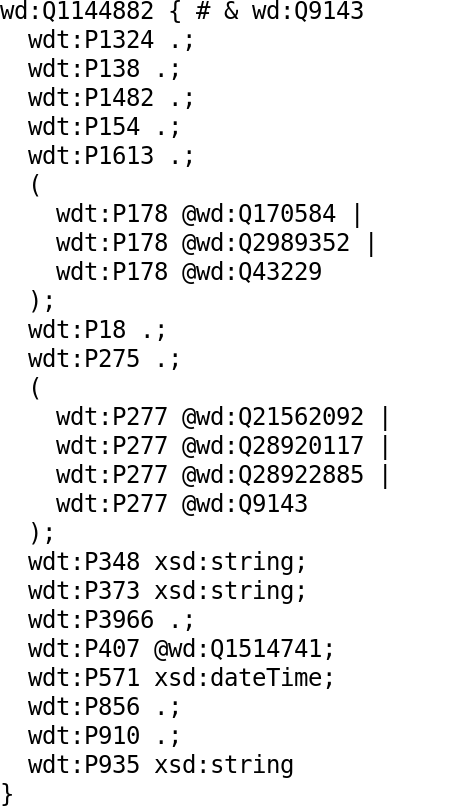
\includegraphics[trim={0 2.5cm 0 0},clip]{screenshots/shexc-no-syntax-highlighting}
    \caption{
      Excerpt of an inferred schema for Linux distributions.
    }
    \label{fig:shexc-syntax-highlighting-without}
  \end{subfigure}
  \begin{subfigure}[t]{0.45\textwidth}
    \centering
    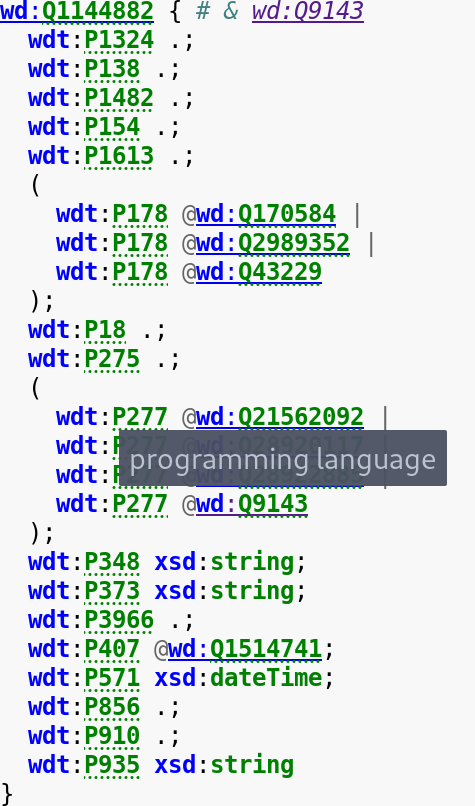
\includegraphics[trim={0 2.5cm 0 0},clip]{screenshots/shexc-with-syntax-highlighting}
    \caption[The same schema with syntax highlighting and the script applied.]{
      The same schema with syntax highlighting and the script applied.
      The cursor is over the \lstinline{P277} \gls{property ID}.
    }
    \label{fig:shexc-syntax-highlighting-with}
  \end{subfigure}
  \caption{
    Screenshots showing the effects of syntax highlighting and the client-side script.
  }
  \label{fig:shexc-syntax-highlighting}
\end{figure}

\section{Toolforge Support}
\label{sec:wdsi:Toolforge}

Since Wikimedia Toolforge runs on a rather old Linux distribution
(Ubuntu 14.04 “Trusty Tahr”, originally released April 2014),
the versions of various software used by \gls{RDF2Graph} and the rest of the inference process
were too outdated to use out-of-the-box.
The response to this was twofold:
to cope with older software versions where feasible,
and to install newer software versions where not.

\Gls{RDF2Graph} required Java 8,
but only Java 7 is installed on Toolforge.
Fortunately, \gls{RDF2Graph} only used Java 8 for syntactic constructs (“lambda” syntax)
and those only sparingly, so it was not too much work to make it compatible with Java 7 again.
Similarly, Apache Jena and Fuseki have required Java 8 for some time already,
but fortunately \gls{RDF2Graph} is compatible with their older versions which support Java 7,
and which could therefore be installed.

On the other hand, there is no obvious way to make the \command{jq}-based part of the data download step
work with \command{jq} version 1.4, which has no general string replacement capabilities.
Therefore, \command{jq} version 1.5 was installed locally into the tool’s home directory –
as was the latest version of \gls{Node.js}, which was similarly outdated.
(The Pygments syntax highlighter mentioned in \cref{sec:wdsi:utilities} was also installed locally,
since \gls{shexc} syntax support is not yet available in any released version.)

Full installation instructions may be found in the \filename{README} file of the source code repository.
